\documentclass{article}
\usepackage[T2A]{fontenc}
\usepackage[russian]{babel}
\usepackage[utf8]{inputenc}

%%%%%%%%%%%%%%%%%%%%%%%%%%%% ДОП.СИМВОЛЫ  %%%%%%%%%%%%%%%%%%%%%%%%%%%%%%%%
\usepackage{amsmath}
\usepackage{amssymb}
\usepackage{latexsym}
\usepackage{amsfonts}
\usepackage{extarrows}
\usepackage{braket}
\usepackage{MnSymbol}
\usepackage{mathtools}
\usepackage{commath}

\DeclarePairedDelimiter{\ceil}{\lceil}{\rceil}
\DeclarePairedDelimiter{\floor}{\lfloor}{\rfloor}
%%%%%%%%%%%%%%%%%%%%%%%%%%%%%%%%%%%%%%%%%%%%%%%%%%%%%%%%%%%%%%%%%%%%%%%

%%%%%%%%%%%%%%%%%%%%%%%%%%%%%  ГРАФИКА  %%%%%%%%%%%%%%%%%%%%%%%%%%%%%%%%
%Цвета:
\usepackage{color} 
\usepackage{xcolor}

%Картиночки:
\usepackage{graphicx}
\graphicspath{{pictures/}}
\DeclareGraphicsExtensions{.pdf,.png,.jpg}

%Встроенная графика 
\usepackage{tikz}
\usetikzlibrary{
    shapes.symbols,
    shapes.geometric,
    shadows,arrows.meta,
    graphs
}

\usepackage{flowchart}
%%%%%%%%%%%%%%%%%%%%%%%%%%%%%%%%%%%%%%%%%%%%%%%%%%%%%%%%%%%%%%%%%%%%%%%%

%%%%%%%%%%%%%%%%%%%%%%%%%%%%%% ВЕРСТКА 1 %%%%%%%%%%%%%%%%%%%%%%%%%%%%%%%%%
\usepackage[toc,page]{appendix}
\usepackage{hyperref}
\hypersetup{
    unicode=true,
    colorlinks=true,
    linktoc=all,  
    linkcolor=blue,
}
\usepackage{hhline}
\usepackage{subcaption}
\usepackage{float}
\usepackage{enumitem}
%%%%%%%%%%%%%%%%%%%%%%%%%%%%%%%%%%%%%%%%%%%%%%%%%%%%%%%%%%%%%%%%%%%%%%%%

%%%%%%%%%%%%%%%%%%%%%%%%%%%%%% ВЕРСТКА 2 %%%%%%%%%%%%%%%%%%%%%%%%%%%%%%%%%
% Шрифты - настройки по умолчанию.
\renewcommand{\rmdefault}{cmr}
\renewcommand{\sfdefault}{cmss}
\renewcommand{\ttdefault}{cmtt}

%Формат секции
\makeatletter
\renewcommand{\@seccntformat}[1]{}
\makeatother


%Пробел
\setlength{\parindent}{0pt}
\setlength{\parskip}{3pt}

%Размеры страницы (не забыть подогнать под принтер)
\usepackage[left=2cm,right=2cm,bottom=2cm]{geometry}

%Списки:
\setlist{topsep=1pt, itemsep=0em}
%%%%%%%%%%%%%%%%%%%%%%%%%%%%%%%%%%%%%%%%%%%%%%%%%%%%%%%%%%%%%%%%%%%%%%%%%%%%%%%%%%%%%%%%%%%%

\title{Линейная регрессия}
\author{Ельцов Данил, Михаил Михайлов}

\begin{document}
\maketitle

\tableofcontents

\section*{Резюме}
По датасетам с Kaggle и официальной статистики по COVID-19 в мире была построена регрессионная модель, способная по демографическим данным страны предсказать кривую развития
пандемии в отдельно взятой стране.

На вход модель принимает числовые характеристики конкретной страны, такие как средний возраст, индекс урбанизации и проч. и результатом работы программы являются коэффициенты логистической прямой
\newpage

\section{Постановка задачи}
Предсказать динамику роста новой коронавирусной инфекции в конкретной стране, основываясь на ее географических и демографических особенностях.

\section{Используемые данные}
Был взят \href{https://www.kaggle.com/daniboy370/world-data-by-country-2020}{датасет}, содержащий числовые характеристики самых больших стран с Kaggle. Представляет из себя несколько таблиц одинакового формата: \textbf{id}, \textbf{country}, \textbf{country\_code}, \textbf{feature}

Также был взят \href{https://www.ecdc.europa.eu/en/publications-data/download-todays-data-geographic-distribution-covid-19-cases-worldwide}{датасет}, содержащий официальную статистику по развитию коронавируса в разных странах
.
\section{Описание решения}
\subsection{Идея решения}
В результате анализа темпов развития COVID-19 в различных странах было сделано предположение, что развитие коронавируса в целом происходит согласно логистической кривой. В следствие этого было решено построить регрессионную модель для предсказания \textbf{параметров логистической кривой}.

\subsection{Подготовка данных}
Для начала необходимо было объединить все характеристики стран в один CSV-файл, что легко было сделано с помощью их трех-буквенного кода. Затем мы к каждой стране из этой таблицы сопоставили посчитанные для неё коэффициенты логистической регрессии. В результате получился файл \textbf{clear\_data.csv}, имеющий следующую структуру:
\[\mathrm{(ISO-code|rfactor|Median-age|Sex-ratio|Urbanization -rate)}\]

\subsection{Вычисление коэффициентов}
Дифференциальное уравнение задающее логистическую кривую выглядит следующим образом
\[\frac{dP}{dt} = rP(1-\frac{P}{K})\]
где параметры кривой это:

\begin{itemize}
    \item P - количество зараженных
    \item r - коэффициент роста
    \item K - поддерживающая емкость среды
\end{itemize} 

Поддерживающую емкость среды в различных моделях оценивают как число из промежутка \([0.75P_{max}; P_{max}]\) где \(P_{max}\) --- число жителей в данной стране, поэтому значение \(K\) нас не интересует. Таким образом интересует только коэффициент роста \(r\).

\subsubsection{Теоретический расчет параметров}
Поймем как можно вычислять параметр \(r\). Проведя преобразования над уравнением кривой получаем
\[\frac{dP}{P} = r\left(1 - \frac{P}{K}\right)dt\]
Проведем усреднение, \textit{предположив}, что выражение в скобках будет равно примерно \(\frac{1}{2}\):
\[\braket{\frac{dP}{P}} = \frac{rdt}{2}\]
Теперь положим для удобства приращение \(dt = 1\) (так как мы сами выбираем единицы относительно которых считаем), получим:

\[r = 2 * \frac{1}{n}\sum_{i=1}^{n} \frac{dP_i}{P_i}\]

Где \(P_i, dP_i\) --- общее число больных и число заболевших на \(i\)-ый день.

\subsubsection{Предсказание целевой переменной}

Для предсказания коэффициента $r$ логистической кривой конкретной страны будут использованы её следующие демографические признаки:
\begin{itemize}
    \item sex\_ratio
    \item median\_age
    \item urbanization\_rate
\end{itemize}

\subsection{Построение регрессионной модели}
    После предпосчета параметров регрессии для каждой страны мы запустили обучение модели \href{https://scikit-learn.org/stable/modules/generated/sklearn.linear_model.LinearRegression.html}{LinearRegression} из популярной библиотеки для машинного обучения - \textbf{sklearn}, которая подобрала коэффициенты регрессионной кривой методом наименьших квадратов. 
    
\section{Результаты}

\begin{figure}[h!]
    \centering
    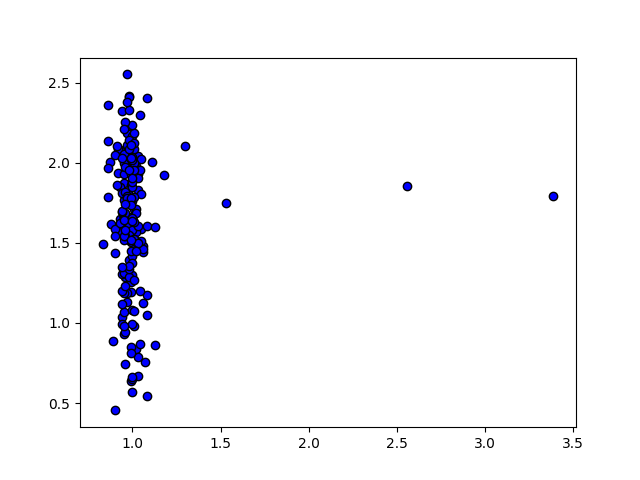
\includegraphics[scale=0.3]{ex.png}
    \caption{Результаты работы регрессии}
    \label{fig1}
\end{figure}

На рисунке \ref{fig1} представлены нормализованные данные (значение \(r\) помножено на 100, рассматриваемые параметры -- минмакс нормализация) и прямая регрессии. Видно, что вообще говоря коэффициент \(r\) не имеет линейной зависимости от исследуемых параметров. Возможно, это связанно с методом подсчета значения \(r\) --- хотя получились вполне реалистичные числа, такой метод подсчета не имеет качественного обоснования. Возможно, это связано с самой природой числа \(r\) и индекс урбанизации, распределение по полу, средний возраст не влияют на значение параметра \(r\) или влияют незначительно. Для проверки роли вклада рассматриваемых параметров в значение \(r\) можно рассмотреть другие параметры

На текущий момент вывод таков --- \textbf{зависимость \(r\) от рассматриваемых параметров не является линейной}.

\begin{itemize}
    \item Подборка датасета - Данил Ельцов, Михаил Михайлов
    \item Анализ данных - Данил Ельцов, Михаил Михайлов
    \item Построение модели, код - Михаил Михайлов
    \item Анализ результатов - Михаил Михайлов
    \item Отчёт - Данил Ельцов, Михаил Михайлов
    \item\href{https://github.com/Desiment/ml-study/blob/main/linear_regression}{Code}
\end{itemize}

\end{document} 

